\documentclass[14pt]{beamer} %Makes presentation
%\documentclass[handout]{beamer} %Makes Handouts
\usetheme{Singapore} %Gray with fade at top
\useoutertheme[subsection=false]{miniframes} %Supppress subsection in header
\useinnertheme{rectangles} %Itemize/Enumerate boxes
\usecolortheme{seagull} %Color theme
\usecolortheme{rose} %Inner color theme

\definecolor{light-gray}{gray}{0.75}
\definecolor{dark-gray}{gray}{0.55}
\setbeamercolor{item}{fg=white}
\setbeamercolor{enumerate item}{fg=dark-gray}

\setbeamertemplate{navigation symbols}{}
%\setbeamertemplate{mini frames}[default]
%\setbeamercovered{dynamics}
\setbeamerfont*{title}{size=\large,series=\bfseries}
\setbeamerfont{footnote}{size=\tiny}

%\setbeameroption{notes on second screen} %Dual-Screen Notes
%\setbeameroption{show only notes} %Notes Output

\setbeamertemplate{frametitle}{\vspace{.5em}\bfseries\insertframetitle}
\newcommand{\heading}[1]{\noindent \textbf{#1}\\ \vspace{1em}}

\usepackage{bbding,color,multirow,times,ccaption,tabularx,graphicx,verbatim,booktabs}
\usepackage{amsmath}
\usepackage{colortbl} %Table overlays
\usepackage[english]{babel}
\usepackage[latin1]{inputenc}
\usepackage[T1]{fontenc}
\usepackage{lmodern}

%\author[]{Thomas J. Leeper}
\institute[]{
  \inst{}%
  Department of Government\\London School of Economics and Political Science
}

\usepackage{tikz}
\usetikzlibrary{shapes,arrows}

\title{Statistical Foundations I}

\date[]{}

\begin{document}

\frame{\titlepage}

\frame{\tableofcontents}

\section[Definition]{What is an experiment?}
\frame{\tableofcontents[currentsection]}

\frame{

\frametitle{Principles of causality}

\begin{enumerate}\itemsep1em
\item \textbf<2->{Correlation/Relationship}
\item \textbf<2->{Nonconfounding}
\item \textbf<2->{Direction (``temporal precedence'')}

\vspace{1em}

\item Mechanism

\vspace{0.5em}

\item Appropriate level of analysis
\end{enumerate}
}

\frame{

\frametitle{Experiments are different}

\begin{enumerate}\itemsep0.75em
\item<2-> Draw causal inferences through \textit{design}
\item<3-> Randomization breaks selection bias and fixes temporal precedence
\item<4-> We don't need to ``control'' for anything
\item<5-> We see ``causal effects'' in the comparison of experimental groups
\end{enumerate}

}


% pieces of an experiment

\frame{

\frametitle{Definitions I}

\begin{itemize}\itemsep0.75em
\item<2-> A randomized experiment, or randomized control trial (RCT), is:
\end{itemize}
	\begin{quote}\small
		The observation of units after, and possibly before, a randomly assigned intervention in a controlled setting, which tests one or more precise causal expectations
	\end{quote}
\begin{itemize}\itemsep0.75em
\item<3-> If we manipulate the thing we want to know the effect of ($X$), and control (i.e., hold constant) everything we do not want to know the effect of ($Z$), the only thing that can affect the outcome ($Y$) is $X$.
\end{itemize}

}


\frame{

\frametitle{Definitions II}

\only<2>{\textbf{Unit}: A physical object at a particular point in time}

\only<3>{\textbf{Treatment}: An intervention, whose effect(s) we wish to assess relative to some other (non-)intervention}

\only<4>{\textbf{Outcome}: The variable we are trying to explain}

\only<5>{
\textbf{Potential outcomes}: The outcome value for each unit that we \textit{would observe} if that unit received each treatment\\

\vspace{1em}

Multiple potential outcomes for each unit, but we only observe one of them

}

\only<6>{\textbf{Causal effect}: The comparisons between the unit-level potential outcomes under each intervention\\

\vspace{1em}

\textit{This is what we want to know!}
}

}

\frame{

\frametitle{Example}

\only<2>{\textbf{Unit}: Schools in Kenya}

\only<3>{\textbf{Outcome}: Student learning}

\only<4>{\textbf{Treatment}: An additional teacher per class, reducing effective class size}

\only<5>{
\textbf{Potential outcomes}:

\begin{enumerate}
\item Knowledge in a ``large'' class
\item Knowledge in a ``small class
\end{enumerate}

}

\only<6>{\textbf{Causal effect}: Difference in knowledge between the two conditions
}

}


\frame{

\frametitle{Units}

\begin{itemize}\itemsep1em
\item Units can be almost anything
\item Common units in experimental designs:
	\begin{itemize}
	\item Individual people
	\item Sites (schools, classes, surgeries)
	\item Areas (districts, states)
	\end{itemize}
\item Units are period-specific
	\begin{itemize}
	\item Randomization can occur over time
	\end{itemize}
\end{itemize}

}



\frame{

\frametitle{Outcomes}

\begin{itemize}\itemsep0.5em
\item Experiments can have many outcome concepts/measures
\item Quite common to think about just one at a time
\item Outcomes can be anything that:
	\begin{itemize}
	\item Is observable/measurable
	\item Can be measured at the level of randomization or lower
	\end{itemize}
\end{itemize}

}


\frame{

\frametitle{Treatments}

\begin{itemize}\itemsep0.5em
\item Synonyms: manipulation, intervention, factor, condition, cell
\item Treatments are operationalizations of independent variables in a causal theory
\item A set of treatments generates observable variation in $X$
\end{itemize}
}


\frame{

\frametitle{Developing Treatments}

\begin{itemize}\itemsep1em
\item From theory, we derive testable hypotheses\\

	\begin{itemize}
	\item Hypotheses are expectations about differences in outcomes across levels of a putatively causal variable
	\item In an experiment, an hypothesis must be testable by an ATE
	\end{itemize}

\item The experimental manipulations induce variation in the causal variable that enable tests of the hypotheses
\end{itemize}

}


\frame{

\frametitle{{\normalsize Example: Framing and Attention\footnote{Walgrave, Sevenans, Van Camp, Loewen (2017) -- ``What Draws Politicians' Attention? An Experimental Study of Issue Framing and its Effect on Individual Political Elites''}}}

\small

\begin{itemize}
\item Theory: Presentation of information affects politicians' attention
\item Hypothesis:
	\begin{itemize}\footnotesize
	\item Information framed as a conflict draws more attention from political elites than information not framed as a conflict.
	\end{itemize}
\item Manipulation:
	\begin{itemize}\footnotesize
	\item Control group: Presentation of headline information
	\item Treatment group: Same information presented as conflict
	\end{itemize}
\item Outcome:
	\begin{itemize}
	\item How likely are legislators to read full article
	\end{itemize}
\end{itemize}

}


\frame{

\frametitle{{\normalsize Ex.: Presence/Absence}}

\small

\begin{itemize}\itemsep0.5em
\item Theory: Legislators vote in line with constituents' preferences
\item Hypothesis: Exposure to a poll of constituent views shifts legislative votes.
\item Manipulation:
	\begin{itemize}\small 
	\item Control group receives no polling information. 
	\item Treatment group receives a letter containing polling information.
	\end{itemize}
\item Outcome:
	\begin{itemize}
	\item How legislators vote on relevant piece of legislation
	\end{itemize}
\end{itemize}

}


\frame{

\frametitle{{\normalsize Ex.: Levels/doses}}

\small

\begin{itemize}\itemsep-0.2em
\item Theory: Legislators vote in line with constituents' preferences
\item Hypothesis: Exposure to a poll of constituent views shifts legislative votes.
\item Manipulation:
	\begin{itemize}\small 
	\item Control group receives no polling information. 
	\item Treatment group 1 receives a letter containing polling information.
	\item Treatment group 2 receives two letters containing polling information.
	\item etc.
	\end{itemize}
\item Outcome:
	\begin{itemize}
	\item How legislators vote on relevant piece of legislation
	\end{itemize}
\end{itemize}

}


\frame{

\frametitle{{\normalsize Ex.: Qualitative variation}}

\small

\begin{itemize}
\item Theory: Legislators vote in line with constituents' preferences
\item Hypothesis: Exposure to a poll of constituent views shifts legislative votes.
\item Manipulation:
	\begin{itemize}\small 
	\item Control group receives no polling information. 
	\item Treatment group 1 receives a letter containing polling information suggesting public support.
	\item Treatment group 2 receives a letter containing polling information suggesting public opposition.
	\end{itemize}
\item Outcome:
	\begin{itemize}
	\item How legislators vote on relevant piece of legislation
	\end{itemize}
\end{itemize}

}

\frame{

\frametitle{Treatments Test Hypotheses!}

\begin{itemize}\itemsep1em
\item<2-> Derive experimental design from hypotheses
\item<3-> Experimental ``factors'' are expressions of hypotheses as randomized groups
\item<4-> What intervention each group receives depends on hypotheses
	\begin{itemize}
	\item presence/absence
	\item levels/doses
	\item qualitative variations
	\end{itemize}
\end{itemize}

}

\frame{\huge\vskip20pt\textbf{Questions?}}


\frame{

\frametitle{Complexities}

\begin{itemize}\itemsep0.5em
\item Experiments can have additional ``moving parts''
	\begin{itemize}
	\item Control groups and placebo groups
	\item Pre-treatment outcome measurement
	\item Within-subjects design features
	\item Repeated measures of outcomes
	\item Cluster randomization
	\item Sampling from a population
	\item \dots
	\end{itemize}
\item None of these are \textit{necessary} for causal inference
\end{itemize}

}


\section{Treatment Effects}
\frame{\tableofcontents[currentsection]}

\frame{

\frametitle{The Fundamental Problem of Causal Inference!}

\begin{itemize}\itemsep1em
\item Units have multiple potential outcomes
\item We can only observe one of them!
\item Thus we never know the individual-level causal effect of a treatment for a given unit
\end{itemize}

}

\frame{

\frametitle{Two Solutions!}

\begin{enumerate}\itemsep1em
\item Assume units are all ``homogeneous'' (i.e., identical)
\item Randomly assign units to treatments and compare \textit{average} outcomes
\end{enumerate}

}


\frame{
	\frametitle{``The Perfect Doctor''}

\small
\begin{center}
\begin{tabular}{ccc}
Unit & $Y_0$ & $Y_1$ \\ \hline 
1 & ? & ? \\
2 & ? & ? \\
3 & ? & ? \\
4 & ? & ? \\
5 & ? & ? \\
6 & ? & ? \\
7 & ? & ? \\
8 & ? & ? \\ \hline
\textbf{Mean} & \textbf{?} & \textbf{?} \\
\end{tabular}
\end{center}
}

\frame{
	\frametitle{``The Perfect Doctor''}

\small
\begin{center}
\begin{tabular}{ccc}
Unit & $Y_0$ & $Y_1$ \\ \hline 
1 & ? & 14 \\
2 & 6 & ? \\
3 & 4 & ? \\
4 & 5 & ? \\
5 & 6 & ? \\
6 & 6 & ? \\
7 & ? & 10 \\
8 & ? & 9 \\ \hline
\textbf{Mean} & \textbf{5.4} & \textbf{11} \\
\end{tabular}
\end{center}
}

\frame{
	\frametitle{``The Perfect Doctor''}

\small
\begin{center}
\begin{tabular}{ccc}
Unit & $Y_0$ & $Y_1$ \\ \hline 
1 & 13 & 14 \\
2 & 6 & 0 \\
3 & 4 & 1 \\
4 & 5 & 2 \\
5 & 6 & 3 \\
6 & 6 & 1 \\
7 & 8 & 10 \\
8 & 8 & 9 \\ \hline
\textbf{Mean} & \textbf{7} & \textbf{5} \\
\end{tabular}
\end{center}
}



\frame{
	\frametitle{Experimental Inference I}
	\begin{itemize}\itemsep1em
    	\item<1-> We cannot see individual-level causal effects
    	\item<2-> We can see \textit{average causal effects}
    		\begin{itemize}
        		\item<2-> Ex.: Average difference in cancer between those who do and do not smoke
    		\end{itemize}
    	\item<3-> We want to know: $TE_i = Y_{1i} - Y_{0i}$
	\end{itemize}
}

\frame{
	\frametitle{Experimental Inference II}
	\begin{itemize}\itemsep1em
		\item<1-> We want to know: $TE_i = Y_{1i} - Y_{0i}$
		\item<2-> We can average: $ATE = E[Y_{1i} - Y_{0i}] = E[Y_{1i}] - E[Y_{0i}]$
		\item<3-> But we still only see one potential outcome for each unit:\\ \vspace{1em}
    		$ATE_{naive} = E[Y_{1i} | X = 1] - E[Y_{0i} | X = 0]$
    	\item<4-> Is this what we want to know?
	\end{itemize}
}


\frame{
	\frametitle{Experimental Inference III}
	\small
	\begin{itemize}\itemsep1em
	\item What we want and what we have:
		\begin{align}
		ATE & = E[Y_{1i}] - E[Y_{0i}] \\[1em]
		ATE_{naive} & = E[Y_{1i} | X = 1] - E[Y_{0i} | X = 0]
		\end{align}		
	\item<2-> Are the following statements true?\\
  		\begin{itemize}\itemsep0.5em
      		\item<2-> $E[Y_{1i}] = E[Y_{1i} | X = 1]$
      		\item<2-> $E[Y_{0i}] = E[Y_{0i} | X = 0]$
  		\end{itemize}
  	\item<3-> Not in general!
  	\end{itemize}
}

\frame{
	\frametitle{Experimental Inference IV}
	\small
	\begin{itemize}\itemsep0.5em
    	\item Only true when both of the following hold:
    	\begin{align}
    	E[Y_{1i}] = E[Y_{1i} | X = 1] = E[Y_{1i} | X = 0]\\
    	E[Y_{0i}] = E[Y_{0i} | X = 1] = E[Y_{0i} | X = 0]
    	\end{align}
    	\item In that case, potential outcomes are \textit{independent} of treatment assignment
		\item If true, then:
    	\begin{align*}
    	ATE_{naive} & = E[Y_{1i} | X = 1] - E[Y_{0i} | X = 0] \tag{5}\\
    	& = E[Y_{1i}] - E[Y_{0i}]\\
    	& = ATE
    	\end{align*}
	\end{itemize}
}

\frame{
	\frametitle{Experimental Inference V}
	\small
	\begin{itemize}\itemsep0.5em
    	\item This holds in experiments because of randomization, which is a special, physical process of unpredictable sorting\footnote{Not ``random'' in the casual, everyday sense of the word}
    		\begin{itemize}
        		\item Units differ only in what side of coin was up
        		\item Experiments randomly reveal potential outcomes
        		\item Randomization balances $Z$ \textit{in expectation}
    		\end{itemize}
	\end{itemize}
}


\frame{}

\frame{
\frametitle{Experimental Analysis I}
\small
\begin{itemize}\itemsep0.5em
\item The statistic of interest in an experiment is the \textit{(sample) average treatment effect} (SATE)
\item This boils down to being a mean-difference between two groups:
	\begin{equation}
	\widehat{SATE} = \left(\frac{1}{n_1}\sum_{i=1}^{n_1} Y_{1i}\right) - \left(\frac{1}{n_0}\sum_{i=1}^{n_0} Y_{0i}\right)
	\end{equation}
\item<2-> Experiments do not require ``controlling for'' anything, if randomization occurred successfully
\end{itemize}
}



\frame[label=tidy]{

\frametitle{Experimental Data Structures}

An experimental data structure looks like:

\small

\begin{center}
\begin{tabular}{ccc}
\texttt{unit} & \texttt{treatment} & \texttt{outcome} \\ \hline 
A & 0 & 5 \\
B & 0 & 7 \\
C & 0 & 9 \\
D & 0 & 4 \\
E & 1 & 9 \\
F & 1 & 4 \\
G & 1 & 13 \\
H & 1 & 12 \\ \hline
\end{tabular}
\end{center}

}




\frame{\huge\vskip20pt\textbf{Questions?}}




\section{Statistical Inference}
\frame{\tableofcontents[currentsection]}


\frame{
\frametitle{Experimental Analysis I}
	\small
\begin{itemize}\itemsep0.5em
\item We don't just care about the size of the SATE. We also want to measure it precisely and know whether it is significantly different from zero (i.e., different from no effect/difference)
\item To know that, we need to estimate the \textit{variance} of the SATE
\item The variance is influenced by:
	\begin{itemize}
	\item Total sample size
	\item Variance of the outcome, $Y$
	\item Relative size of each treatment group
	\item ``Advanced'' design features
	\end{itemize}
\end{itemize}
}


\frame{
\frametitle{Experimental Analysis II}
\begin{itemize}\itemsep1em
\item Formula for the variance of the SATE is:\\

\vspace{0.5em}

$\widehat{Var}(SATE) = \left(\dfrac{\widehat{Var}(Y_0)}{n_0}\right) + \left(\dfrac{\widehat{Var}(Y_1)}{n_1}\right)$

	\begin{itemize}
	\item $\widehat{Var}(Y_0)$ is control group variance
	\item $\widehat{Var}(Y_1)$ is treatment group variance
	\end{itemize}

\item We often express this as the \textit{standard error} of the estimate:\\

\vspace{0.5em}

$\widehat{SE}_{SATE} = \sqrt{\frac{\widehat{Var}(Y_0)}{n_0} + \frac{\widehat{Var}(Y_1)}{n_1}}$

\end{itemize}
}

\frame{

\frametitle{Intuition about Variance}

\begin{itemize}\itemsep1em
\item Bigger sample $\rightarrow$ smaller SEs

\item Smaller variance $\rightarrow$ smaller SEs

\item Efficient use of sample size:
	\begin{itemize}
	\item When treatment group variances equal, equal sample sizes are most efficient
	\item When variances differ, sample units are better allocated to the group with higher variance in $Y$
	\end{itemize}
\end{itemize}

}


\frame{

\frametitle{Statistical Inference}

\begin{itemize}\itemsep1em
\item To assess whether an effect differs from zero, we need to know the sampling distribution of the ATE
\item Two major ways to do this:
	\begin{enumerate}
	\item Assume a parametric distribution (e.g., t-test)
	\item Randomization inference
	\end{enumerate}
\item In large samples, the latter approaches the former
\end{itemize}

}


\frame{

\frametitle{Randomization Inference I}

\begin{itemize}\itemsep1em
\item The randomization (or permutation) distribution is an empirical sampling distribution
\item It conveys the variation we would observe in $\widehat{ATE}$ if a null hypothesis, $H_0: ATE = 0$ was true
\item If this null hypothesis is true, then treatment had no effect; the variation in permuted ATEs therefore only reflects sampling variance
\end{itemize}
}


\frame{

\small

\begin{center}
\begin{tabular}{ccc}
\texttt{unit} & \texttt{treatment} & \texttt{outcome} \\ \hline 
A & 0 & 5 \\
B & 0 & 7 \\
C & 0 & 9 \\
D & 0 & 4 \\
E & 1 & 9 \\
F & 1 & 4 \\
G & 1 & 13 \\
H & 1 & 12 \\ \hline
\end{tabular}
\end{center}

$\widehat{ATE} = 3.25$

}

\frame{

\small

\begin{center}
\begin{tabular}{ccc}
\texttt{unit} & \texttt{treatment} & \texttt{outcome} \\ \hline 
A & 0 & 5 \\
B & 1 & 7 \\
C & 0 & 9 \\
D & 1 & 4 \\
E & 0 & 9 \\
F & 1 & 4 \\
G & 0 & 13 \\
H & 1 & 12 \\ \hline
\end{tabular}
\end{center}

$\widehat{ATE} = -1.5$

}

\frame{

\small

\begin{center}
\begin{tabular}{ccc}
\texttt{unit} & \texttt{treatment} & \texttt{outcome} \\ \hline 
A & 1 & 5 \\
B & 1 & 7 \\
C & 0 & 9 \\
D & 0 & 4 \\
E & 1 & 9 \\
F & 0 & 4 \\
G & 0 & 13 \\
H & 1 & 12 \\ \hline
\end{tabular}
\end{center}

$\widehat{ATE} = 0.75$
}

\frame{

\frametitle{Randomization Distribution}

\begin{center}
\begin{tabular}{cr}
\texttt{Randomization} & \texttt{ATE} \\ \hline 
1 & 3.25 \\
2 & -1.50 \\
3 & 0.75 \\
4 & \dots \\
\dots & \dots  \\ \hline
\end{tabular}
\end{center}

In a two-condition experiment, the number of possible permutations is given by ${n}\choose{n_1}$

}


\frame{

\frametitle{Randomization Inference II}

Randomization inference works as follows:

\begin{enumerate}\itemsep0.5em
\item Generate every possible randomization scheme
	\begin{itemize}
	\item Or sample from all possible randomizations
	\end{itemize}
\item Calculate $ATE$ under each randomization
\item The distribution of those estimates is the randomization distribution
\item Its variance is $\widehat{Var}(ATE)$
\item Proportion of values further from 0 than the observed $\widehat{ATE}$ is the p-value for a test of the null hypothesis ($H_0: ATE = 0$)
\end{enumerate}

}

\frame{
\begin{center}
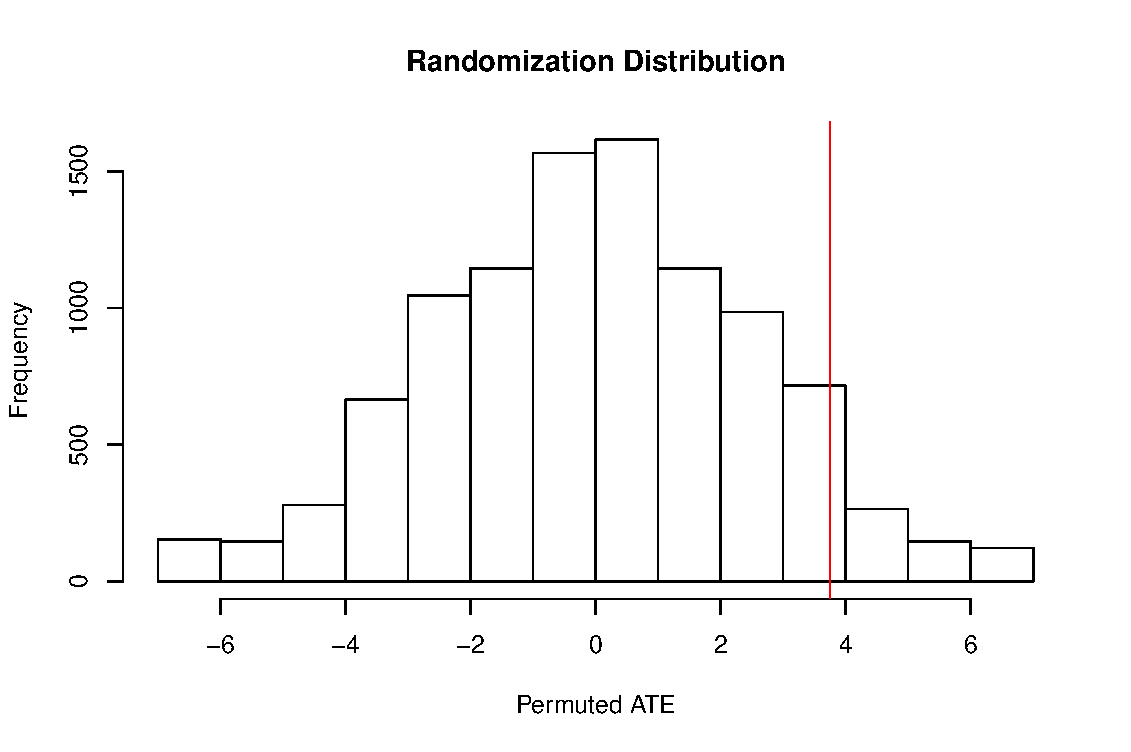
\includegraphics[width=\textwidth]{images/randomization}
\end{center}
}



\begin{frame}[fragile]

\frametitle{Randomization Inference in R}

\footnotesize

\begin{verbatim}
# construct data
d <- data.frame(x = c(0,0,0,0,1,1,1,1), 
                y = c(5,7,9,4,11,4,13,12))

# calculate ATE from each randomization
set.seed(1)    # set random number seed
n <- 10000     # number of randomizations
rd <- replicate(n, coef(lm(d$y ~ sample(d$x, 8)))[2L])

# visualize the randomization distribution
hist(rd)
abline(v = coef(lm(y~x, data = d))[2L], col = "red")

# one-tailed significance test
sum(rd >= coef(lm(y ~ x, data = d))[2L])/n
# two-tailed significance test
sum(abs(rd) >= coef(lm(y ~ x, data = d))[2L])/n
\end{verbatim}

\end{frame}


\begin{frame}[fragile]

\frametitle{Parametric Analysis Stata/R}

R:\small
\begin{verbatim}
t.test(outcome ~ treatment, data = data)
lm(outcome ~ factor(treatment), data = data)
\end{verbatim}

\vspace{1em}

Stata:\small
\begin{verbatim}
ttest outcome, by(treatment)
reg outcome i.treatment
\end{verbatim}

\end{frame}


\frame{\huge\vskip20pt\textbf{Questions?}}


\appendix
\frame{}

\end{document}
